\documentclass[letterpaper,conference]{IEEEtran}
\ifCLASSINFOpdf
	\usepackage[pdftex]{graphicx}
	\graphicspath{{./figures/}}
	\DeclareGraphicsExtensions{.pdf,.jpeg,.jpg,.png}
\else
	\usepackage[dvips]{graphicx}
	\graphicspath{{./figures/}}
	\DeclareGraphicsExtensions{.eps}
\fi

\usepackage[cmex10]{amsmath}
\interdisplaylinepenalty=2500
\usepackage{dblfloatfix}
\usepackage{url}

% *** SUBFIGURE PACKAGES ***
\ifCLASSOPTIONcompsoc
  \usepackage[caption=false,font=normalsize,labelfont=sf,textfont=sf]{subfig}
\else
  \usepackage[caption=false,font=footnotesize]{subfig}
\fi
% subfig.sty, written by Steven Douglas Cochran, is the modern replacement
% for subfigure.sty, the latter of which is no longer maintained and is
% incompatible with some LaTeX packages including fixltx2e. However,
% subfig.sty requires and automatically loads Axel Sommerfeldt's caption.sty
% which will override IEEEtran.cls' handling of captions and this will result
% in non-IEEE style figure/table captions. To prevent this problem, be sure
% and invoke subfig.sty's "caption=false" package option (available since
% subfig.sty version 1.3, 2005/06/28) as this is will preserve IEEEtran.cls
% handling of captions.
% Note that the Computer Society format requires a larger sans serif font
% than the serif footnote size font used in traditional IEEE formatting
% and thus the need to invoke different subfig.sty package options depending
% on whether compsoc mode has been enabled.
%
% The latest version and documentation of subfig.sty can be obtained at:
% http://www.ctan.org/tex-archive/macros/latex/contrib/subfig/

\IEEEoverridecommandlockouts

% Title Page
\title{A Snapshot of Desktop and Mobile Web Page Characteristics}
\author{\IEEEauthorblockN{Troy Johnson}
	\IEEEauthorblockA{Dept. of Computer Science\\
		Central Michigan University\\
		Mount Pleasant, MI 48859\\
		Email: johns4ta@cmich.edu}
	\and
	\IEEEauthorblockN{Patrick Seeling}
	\IEEEauthorblockA{Dept. of Computer Science\\
		Central Michigan University\\
		Mount Pleasant, MI 48859\\
		Email: pseeling@ieee.org}
}


\begin{document}
\maketitle

\begin{abstract}
In this paper, we evaluate the differences of the number of objects comprising and sizes of web pages as delivered to desktop and mobile web clients based on a large publicly available dataset of initial page views.

\end{abstract}

\begin{IEEEkeywords}
	Mobile communication, traffic modeling, data communications
\end{IEEEkeywords}

\section{Introduction}

Smart mobile devices with ubiquitous connectivity have become popular worldwide. 
Cisco, Inc. predicts that this will result in steady growth of mobile data for years to come~\cite{Ci13}.
As mobile users employ their always-present devices to access web-based services, additional predictions include a shift of the main access of the world wide web from fixed desktop to mobile clients. 
This results in past studies focusing on desktop client web access, such as \cite{BaCr98}, not reflecting the current state of the web anymore.

To address these changes, more recent studies have found that significant amounts of data traffic can be saved for providers through caching~\cite{IhPa11}.
Investigating the complexity of web pages, the number of loaded objects were found to positively correlate with the web page load times~\cite{BuMaSe13}. 
Furthermore, in their evaluation, the authors found that mobile and non-landing web pages tend to exhibit less complexity.
devices.

%In a recent overview of the battery impact that different web page elements have on the power consumption of mobile  devices, the different elements of web sites were found to contribute differently to the power consumption, see~\cite{ThAgNiBoSi12}.
%For a set of popular web pages, an energy profiling for the different elements of web pages was performed that identified Java Script and CSS as the main culprits for the power consumption when browsers are rendering mobile web pages.
%The composition in addition to the number of objects and bytes overall hence have a direct relation to the web-related performance of mobile devices.

In this paper, we evaluate the difference and similarities of web pages as they were accessed with a desktop and mobile (iphone) client with respect to sizes, number of requests, and caching abilities.
In the following section, we describe the underlying dataset and data gathering procedures. We then describe the high-level characteristics and approximations through distributions.
We conclude with an outlook on future works.

\section{Web Page Dataset}
We utilize the \url{httparchive.org}~\cite{ht13} publicly dataset of captured web performance metrics, which is publicly available. 
The dataset is generated from initial client views (eliminating caching) of a broad set of web sites. 
While the project gathers the statistics of landing pages, in conjunction with the observations in~\cite{BuMaSe13}, these can be seen as representative upper boundaries of the evaluated characteristics.
We utilize the fixed and mobile datasets available for Oct. 1st, 2013. 
We pre-process the dataset to only contain web sites that are present in both sets and hence represent a comparable subset. 
Even with this pre-processing, we evaluate the characteristics of 4779 web sites.




\section{Distribution Fitting}
In the following, we evaluate the possibility to fit the individual web page statistics for the number of requests and web page sizes. 
We utilized the EasyFit distribution fitting software~\cite{Ma13} to evaluate the underlying distributions. 
We find that for both, the General Gamma Distribution provides as reasonable fit of the discovered fundamental characteristics (while noting that other distributions might individually provide a similarly good fit). 
We illustrate the fitted distributions in Figures~\ref{fig:reqs} and \ref{fig:bytes} for requests and sizes, respectively.
\begin{figure}[]
	\centering
	\subfloat[Number of requests]{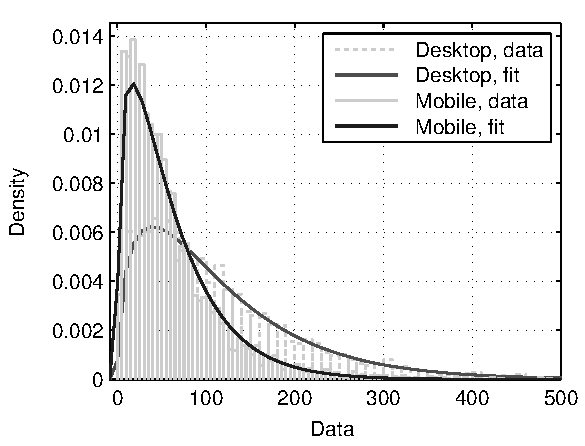
\includegraphics[width=.45\textwidth]{demo}}
	\label{fig:freqs}
	
	\subfloat[Bytes per web page]{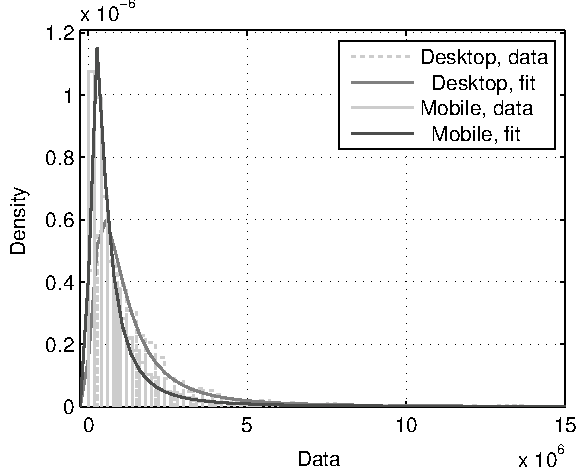
\includegraphics[width=.45\textwidth]{demo-2}}
	\label{fig:mreqs}
	\caption{General distribution fitting for number of object requests (Gamma distribution) and web page sizes (Generalized Extreme Value distribution).\label{fig:reqs}}
\end{figure}

\begin{figure}[t]
	\centering
	\subfloat[Desktop client]{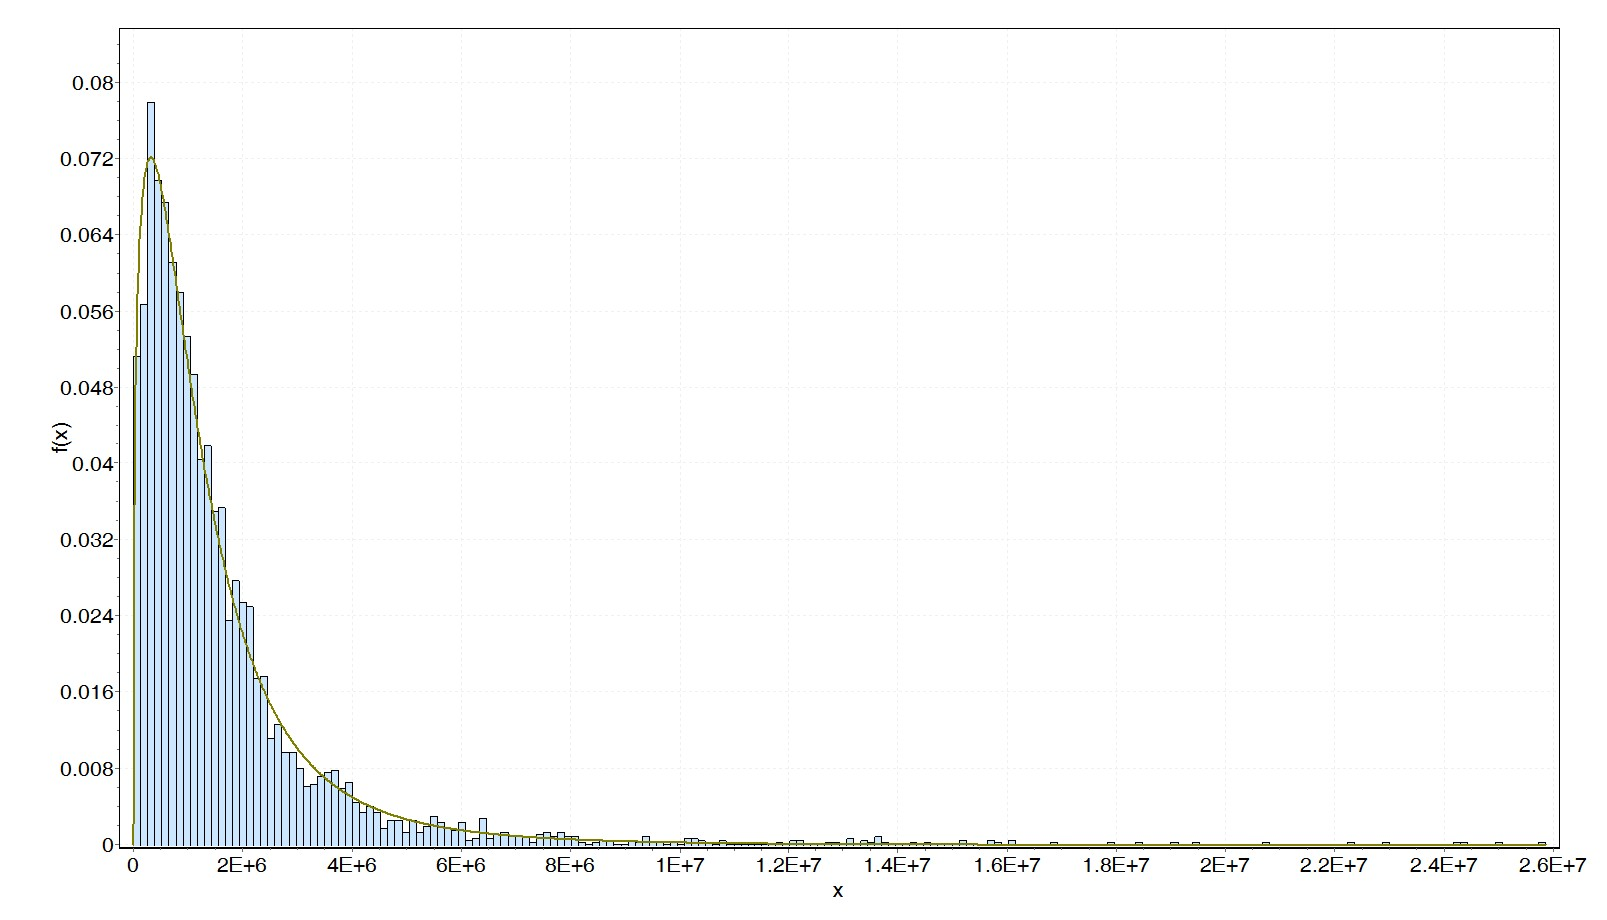
\includegraphics[width=.4\textwidth]{fbytes}}
	\label{fig:fbytes}

	\subfloat[Mobile client]{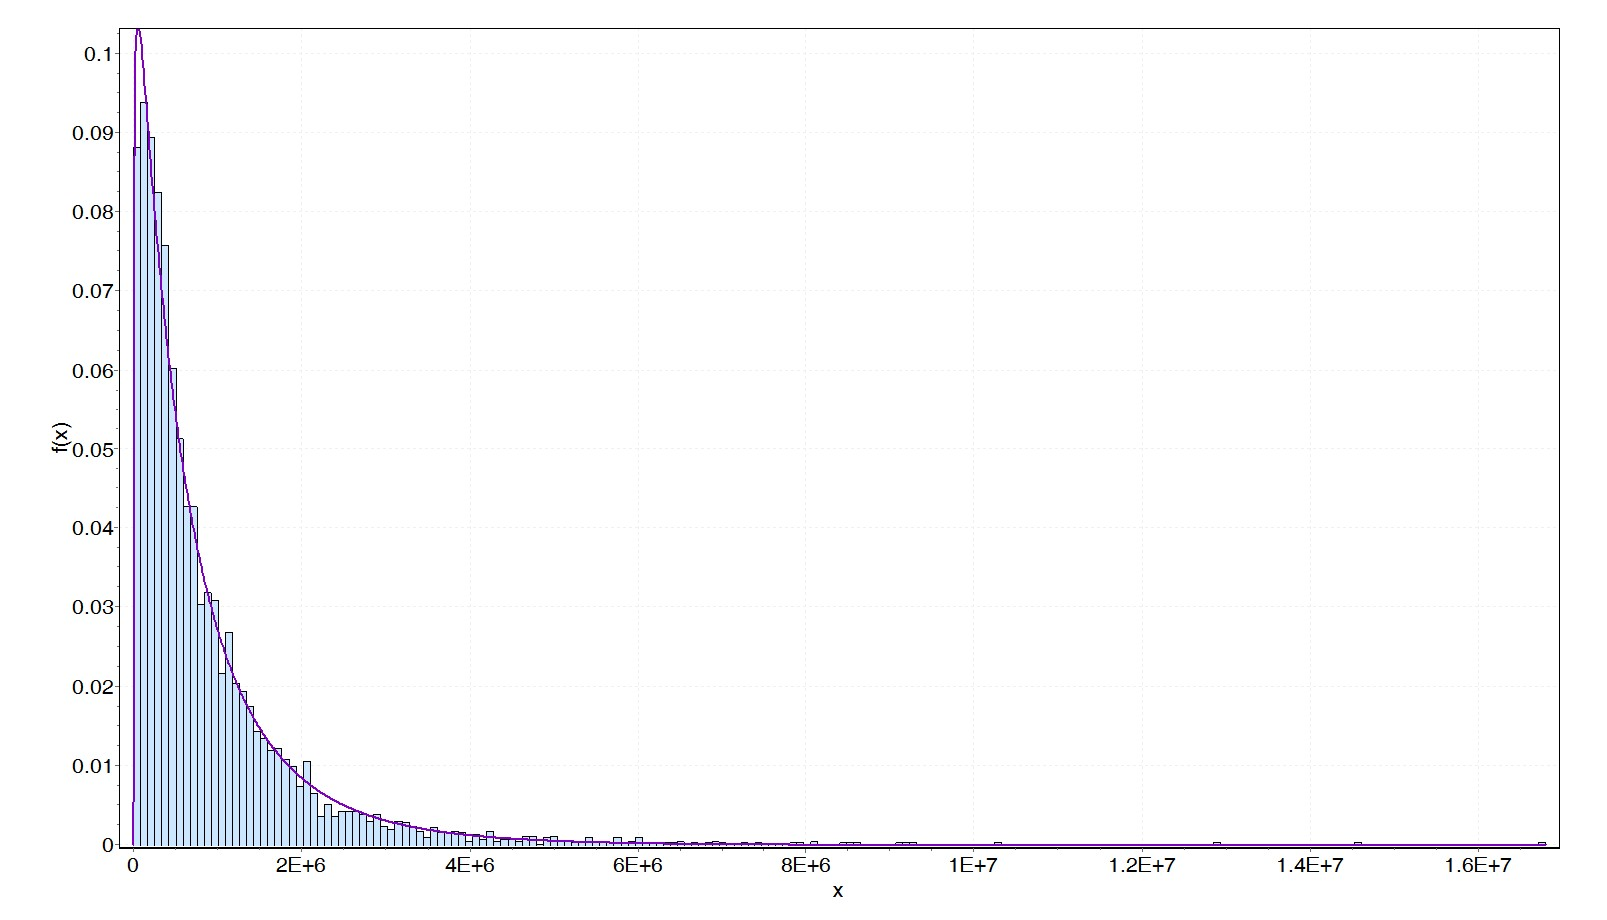
\includegraphics[width=.4\textwidth]{mbytes}}
	\label{fig:mbytes}
	\caption{General Gamma distribution fitting for web page sizes (with 200 illustrated bins).\label{fig:bytes}}
\end{figure}
QQ plots (omitted due to page limits) indicate that the tails exhibit increasing deviations, but the lower ends with the majority of observations are fitted well.

\section{Conclusion}
The increasing importance of web access using mobile devices triggers additional challenges for networks and  
investigating the underlying characteristics and differences between fixed and mobile client web access can yield important insights for optimization and modeling of today's web traffic. 
We found that there is a strong similarity between the access modes for ($i$) sizes per request and ($ii$) the amount of objects that can be cached while the desktop versions exhibit ($iii$) approximately twice the size and ($iv$) twice the number of objects. In the future, we will investigate the potential for detailed modeling of the size and request distributions as well as the possibility for correlations between objects that are cacheable and sizes.

%\section*{Acknowledgment}
%This work was supported in part by an Early Career grant from the Office of Research and Sponsored Programs at Central Michigan University.

%\bibliographystyle{IEEEtran}
%\bibliography{httparchive}

% Generated by IEEEtran.bst, version: 1.13 (2008/09/30)
\begin{thebibliography}{1}
	\providecommand{\url}[1]{#1}
	\csname url@samestyle\endcsname
	\providecommand{\newblock}{\relax}
	\providecommand{\bibinfo}[2]{#2}
	\providecommand{\BIBentrySTDinterwordspacing}{\spaceskip=0pt\relax}
	\providecommand{\BIBentryALTinterwordstretchfactor}{4}
	\providecommand{\BIBentryALTinterwordspacing}{\spaceskip=\fontdimen2\font plus
		\BIBentryALTinterwordstretchfactor\fontdimen3\font minus
		\fontdimen4\font\relax}
	\providecommand{\BIBforeignlanguage}[2]{{%
			\expandafter\ifx\csname l@#1\endcsname\relax
			\typeout{** WARNING: IEEEtran.bst: No hyphenation pattern has been}%
			\typeout{** loaded for the language `#1'. Using the pattern for}%
			\typeout{** the default language instead.}%
			\else
			\language=\csname l@#1\endcsname
			\fi
			#2}}
	\providecommand{\BIBdecl}{\relax}
	\BIBdecl
	
	\bibitem{Ci13}
	\BIBentryALTinterwordspacing
	Cisco, Inc., ``Cisco visual networking index: Forecast and methodology,
	2012--2017,'' Tech. Rep., may 2013. [Online]. Available:
	\url{http://www.cisco.com/en/US/solutions/collateral/ns341/ns525/ns537/ns705/ns827/white_paper_c11-481360.pdf}
	\BIBentrySTDinterwordspacing
	
	\bibitem{BaCr98}
	\BIBentryALTinterwordspacing
	P.~Barford and M.~Crovella, ``Generating representative web workloads for
	network and server performance evaluation,'' \emph{SIGMETRICS Perform. Eval.
		Rev.}, vol.~26, no.~1, pp. 151--160, Jun. 1998. [Online]. Available:
	\url{http://doi.acm.org/10.1145/277858.277897}
	\BIBentrySTDinterwordspacing
	
	\bibitem{IhPa11}
	\BIBentryALTinterwordspacing
	S.~Ihm and V.~S. Pai, ``Towards understanding modern web traffic,'' in
	\emph{Proceedings of the 2011 ACM SIGCOMM conference on Internet measurement
		conference}, ser. IMC '11.\hskip 1em plus 0.5em minus 0.4em\relax New York,
	NY, USA: ACM, 2011, pp. 295--312. [Online]. Available:
	\url{http://doi.acm.org/10.1145/2068816.2068845}
	\BIBentrySTDinterwordspacing
	
	\bibitem{BuMaSe13}
	M.~Butkiewicz, H.~Madhyastha, and V.~Sekar, ``Characterizing web page
	complexity and its impact,'' \emph{Networking, IEEE/ACM Transactions on},
	vol.~PP, no.~99, pp. 1--1, 2013.
	
	\bibitem{ht13}
	\BIBentryALTinterwordspacing
	httparchive.org, ``Http archive (beta),'' July 2013. [Online]. Available:
	\url{http://www.httparchive.org}
	\BIBentrySTDinterwordspacing
	
	\bibitem{Ma13}
	MathWave, ``Easyfit,'' 2013.
	
\end{thebibliography}

\end{document}
